\documentclass[border=4pt]{standalone}
\usepackage{amsmath,amssymb,amsfonts}
\usepackage{xcolor,colortbl,array,booktabs,multirow}
\usepackage{tikz}
\usepackage{pgfplots}
\pgfplotsset{compat=1.16}
\usetikzlibrary{arrows, automata, backgrounds, calendar, chains, decorations,
    matrix, mindmap, patterns, petri, positioning, shadows, shapes.geometric,
    trees, shapes, decorations.pathreplacing, calc, tikzmark, arrows.meta,
    intersections, fit, graphs, quotes, angles, decorations.markings}
\newcommand{\st}{\text{ s.t. }}
\newcommand{\x}{\mathbf{x}}
\renewcommand{\b}{\mathbf{b}}
\renewcommand{\c}{\mathbf{c}}
\newcommand{\A}{\mathbf{A}}
\newcommand{\y}{\mathbf{y}}
\newcommand{\z}{\mathbf{z}}
\newcommand{\R}{\mathbb{R}}
\newcommand{\RR}{\mathbb{R}}
\newcommand{\Z}{\mathbb{Z}}
\newcommand{\ZZ}{\mathbb{Z}}
\newcommand{\npcomplete}{NP-complete}
\providecommand{\true}{\text{TRUE}}
\providecommand{\false}{\text{FALSE}}
\tikzset{vertex/.style={circle,fill=black!25,minimum size=20pt,inner sep=0pt},
    edge/.style={draw,thick,-},weight/.style={font=\small},
    selected vertex/.style={vertex, fill=red!24},
    selected edge/.style={draw,line width=2pt,-,red!50},
    ignored edge/.style={draw,line width=2pt,-,black!20}}
\newcommand{\vect}{\vec}
\providecommand{\ds}{\displaystyle}
\providecommand{\longvect}{\overrightarrow}
\usepackage[normalem]{ulem}
\definecolor{ocre}{RGB}{243,102,25}
\providecommand{\leftB}{\left[}
\providecommand{\rightB}{\right]}
\tikzset{directed/.style={postaction={decorate,decoration={markings,mark=at position .65 with {\arrow{>}}}}},
    directed1/.style={postaction={decorate,decoration={markings,mark=at position .65 with {\arrow{>}}}}}}
\begin{document}
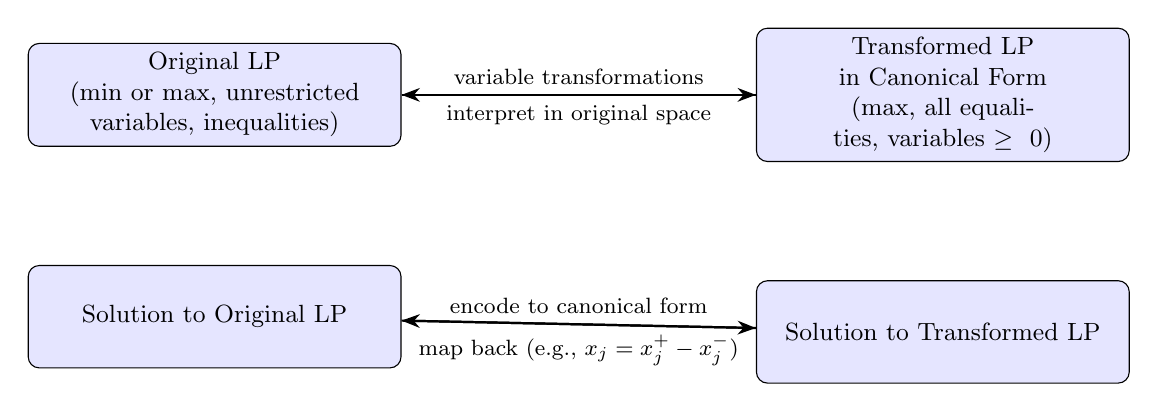
\begin{tikzpicture}[node distance=1.5cm and 4.5cm, every node/.style={font=\small}]
\tikzstyle{box} = [draw, fill=blue!10, rounded corners, text width=4.5cm, minimum height=1.3cm, align=center]
\tikzstyle{arrow} = [-{Stealth}, thick]

% Nodes
\node[box] (original) {Original LP\\ (min or max, unrestricted variables, inequalities)};
\node[box, right=of original] (transformed) {Transformed LP in Canonical Form\\ (max, all equalities, variables $\geq 0$)};
\node[box, below=of original] (origsol) {Solution to Original LP};
\node[box, below=of transformed] (transsol) {Solution to Transformed LP};

% Arrows
\draw[arrow] (original) -- (transformed) node[midway, above] {\footnotesize variable transformations};
\draw[arrow] (transformed) -- (original) node[midway, below] {\footnotesize interpret in original space};

\draw[arrow] (transsol) -- (origsol) node[midway, below] {\footnotesize map back (e.g., $x_j = x_j^+ - x_j^-$)};
\draw[arrow] (origsol) -- (transsol) node[midway, above] {\footnotesize encode to canonical form};

\end{tikzpicture}
\end{document}
